\chapter{Problem Formulation}

Given a string of text, typically a phrase, we are interested in detecting and correcting misspelling errors in the 
typed phrase. This project aims to implement an Error Model, capable of offering corrected candidates to a single 
misspelled word, and a Hidden Markov Model, capable of finding the most likely sequence of candidates for each word in 
a sentence.

The two models work sequentially in a pipeline, but are not strictly dependant on each other, as the Error Model 
acts as a local corrector, and the HMM acts as a maximiser of the probability of the sequences of candidates.

\section{Design Choices}

We have chosen to implement this solution using the English language for various reasons. First of all, great 
majority of material in literature deals with this problem in the English language. \textcolor{red}{Moreover it is a 
simple language, both from a grammatical and a lexical point of view: it lacks in certain symbols, like accents 
and apostrophes, and genres. }
Furthermore all punctuation and special character symbols were not considered, but only letters and sometimes 
numbers. 

We assume that a typed word only depends on the previous one for ease of implementation. As such we will implement a first order HMM. 
If we know the probability of a word given its predecessor, the frequency of each word, and the probability to 
type word $x$ when word $y$ is intended, we have all the necessary ingredients to use Hidden Markov Models.

We also assume that, in our artificial perturbation of words, the number of errors in a word follows a binomial 
distribution depending on the length of the word.

\section{Software}
We have developed the project using the \textbf{Python} programming language, taking advantage of various open-source 
libraries: \textbf{edlib} to compute the sequence of edit operations to transform a word in another one,  
\textbf{networkx} to represent the trellis graph produced by Viterbi's algorithm, \textbf{pandas} to store the 
evaluation results, \textbf{matplotlib} and \textbf{graphviz} to visualize the trellis graph.

We also created a graphical user interface that provides real-time local spell checking and on-demand visualisation of 
the trellis graph. This part is implemented as a native macOS application written in \textbf{Swift} that interacts with 
our Python code using Swift's official Python interoperation.

\begin{figure}[H]
	\centering
	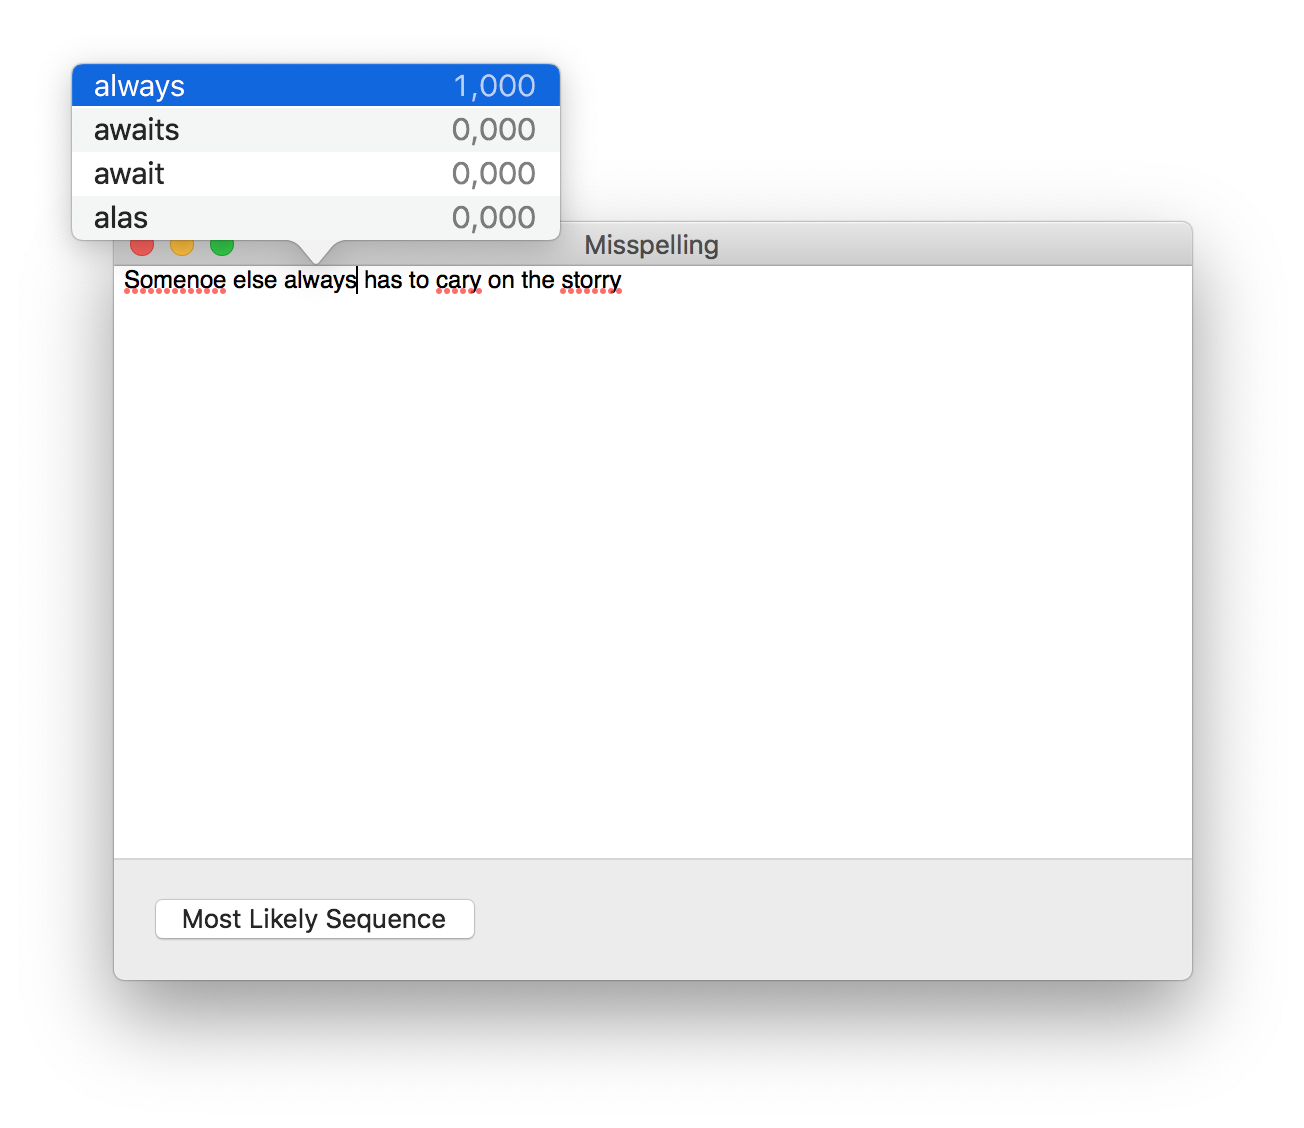
\includegraphics[width=10cm]{ui-candidates.png}
	\caption{Screenshot of the user interface for real-time spell checking}
	\label{fig:noisychannel}
\end{figure}
